% Censoring section for the Survival Analysis book
\section{Understanding Censoring}
\label{sec:understanding-censoring}

Censoring occurs when we have incomplete information about a subject's survival time. It is a fundamental concept in survival analysis as most real-world studies involve some form of censoring. Without accounting for censoring, survival estimates would be biased.

\subsection{Types of Censoring}
\label{subsec:types-of-censoring}

% Censoring visualization using PGFPlots with our publication-grade styles
% To be included in the book

\begin{figure}[htbp]
    \centering
    \begin{tikzpicture}
        \begin{axis}[
            publication,
            width=0.8\textwidth,
            height=0.4\textwidth,
            title={Censoring in Survival Analysis},
            xlabel={Time (months)},
            ylabel={Patient},
            ytick={1,2,3,4,5,6,7,8},
            yticklabels={Patient 1, Patient 2, Patient 3, Patient 4, Patient 5, Patient 6, Patient 7, Patient 8},
            xmin=0,
            xmax=60,
            ymin=0.25,
            ymax=8.75,
            xmajorgrids=true,
            grid style={octonary!20, very thin},
            y dir=reverse,
            legend pos=north east,
            legend style={
                font=\small,
                cells={anchor=west}
            }
        ]
            % Full observation (event occurred)
            \addplot[
                primaryDark,
                thick,
                mark=*,
                mark size=3pt,
                mark options={fill=primaryDark, solid}
            ] coordinates {
                (0,1) (32,1)
            };
            
            % Add death mark
            \node[circle, fill=quaternary, inner sep=2pt] at (axis cs:32,1) {};
            
            % Right-censored observation
            \addplot[
                primaryDark,
                thick,
                mark=none
            ] coordinates {
                (0,2) (48,2)
            };
            
            % Add censoring mark
            \draw[censoringColor, very thick] 
                (axis cs:48-1.5,2-1.5) -- (axis cs:48+1.5,2+1.5);
            \draw[censoringColor, very thick] 
                (axis cs:48-1.5,2+1.5) -- (axis cs:48+1.5,2-1.5);
                
            % Late entry (left truncation)
            \addplot[
                primaryDark,
                thick,
                mark=none,
                dash pattern=on 2pt off 2pt
            ] coordinates {
                (0,3) (12,3)
            };
            
            \addplot[
                primaryDark,
                thick,
                mark=none
            ] coordinates {
                (12,3) (40,3)
            };
            
            % Add death mark
            \node[circle, fill=quaternary, inner sep=2pt] at (axis cs:40,3) {};
            
            % Left truncation and right censoring
            \addplot[
                primaryDark,
                thick,
                mark=none,
                dash pattern=on 2pt off 2pt
            ] coordinates {
                (0,4) (15,4)
            };
            
            \addplot[
                primaryDark,
                thick,
                mark=none
            ] coordinates {
                (15,4) (52,4)
            };
            
            % Add censoring mark
            \draw[censoringColor, very thick] 
                (axis cs:52-1.5,4-1.5) -- (axis cs:52+1.5,4+1.5);
            \draw[censoringColor, very thick] 
                (axis cs:52-1.5,4+1.5) -- (axis cs:52+1.5,4-1.5);
                
            % Interval censoring
            \addplot[
                primaryDark,
                thick,
                mark=none
            ] coordinates {
                (0,5) (25,5)
            };
            
            \addplot[
                primaryDark,
                thick,
                mark=none,
                dash pattern=on 3pt off 3pt
            ] coordinates {
                (25,5) (38,5)
            };
            
            \addplot[
                primaryDark,
                thick,
                mark=none
            ] coordinates {
                (38,5) (45,5)
            };
            
            % Add death mark
            \node[circle, fill=quaternary, inner sep=2pt] at (axis cs:45,5) {};
            
            % Add interval censoring annotation arrow - moved up to avoid overlap with Event type 1
            \draw[->, thin, gray] (32,6.7) -- (32,5.2);
            \node[above, align=center, font=\footnotesize, text=gray] at (32,6.8) {Interval\\censoring};
            
            % Event observed in competing risks
            \addplot[
                primaryDark,
                thick,
                mark=none
            ] coordinates {
                (0,6) (28,6)
            };
            
            % Event 1 mark
            \node[circle, fill=event1Color, inner sep=2pt] at (axis cs:28,6) {};
            
            % Another competing risk event
            \addplot[
                primaryDark,
                thick,
                mark=none
            ] coordinates {
                (0,7) (36,7)
            };
            
            % Event 2 mark
            \node[circle, fill=event2Color, inner sep=2pt] at (axis cs:36,7) {};
            
            % Another competing risk with censoring
            \addplot[
                primaryDark,
                thick,
                mark=none
            ] coordinates {
                (0,8) (50,8)
            };
            
            % Censoring mark
            \draw[censoringColor, very thick] 
                (axis cs:50-1.5,8-1.5) -- (axis cs:50+1.5,8+1.5);
            \draw[censoringColor, very thick] 
                (axis cs:50-1.5,8+1.5) -- (axis cs:50+1.5,8-1.5);
            
            % Add labels with arrows to explain censoring concepts clearly
            % Complete observation
            \draw[->, thin, gray] (33,1.3) -- (33,1.1);
            \node[above, align=center, font=\footnotesize, text=gray] at (33,1.3) {Complete\\observation};
            
            % Right censoring
            \draw[->, thin, gray] (49,2.3) -- (49,2.1);
            \node[above, align=center, font=\footnotesize, text=gray] at (49,2.3) {Right\\censoring};
            
            % Left truncation (Patient 3)
            \draw[->, thin, gray] (6,3.4) -- (6,3.1);
            \node[above, align=center, font=\footnotesize, text=gray] at (6,3.4) {Left\\truncation};
            
            % Event mark
            \draw[->, thin, gray] (41,3.3) -- (41,3.1);
            \node[above, align=center, font=\footnotesize, text=gray] at (41,3.3) {Event};
            
            % Left truncation (Patient 4)
            \draw[->, thin, gray] (10,4.4) -- (14,4.1);
            \node[above, align=center, font=\footnotesize, text=gray] at (10,4.4) {Left\\truncation};
            
            % Right censoring (Patient 4)
            \draw[->, thin, gray] (53,4.3) -- (53,4.1);
            \node[above, align=center, font=\footnotesize, text=gray] at (53,4.3) {Right\\censoring};
            
            % Event after interval
            \draw[->, thin, gray] (46,5.3) -- (46,5.1);
            \node[above, align=center, font=\footnotesize, text=gray] at (46,5.3) {Event};
            
            % Event type 1 - shifted to the right where there's more space
            \draw[->, thin, gray] (40,6.3) -- (29,6.1);
            \node[above, align=center, font=\footnotesize, text=gray] at (40,6.3) {Event\\type 1};
            
            % Event type 2 - shifted to the right where there's more space
            \draw[->, thin, gray] (45,7.3) -- (37,7.1);
            \node[above, align=center, font=\footnotesize, text=gray] at (45,7.3) {Event\\type 2};
            
            % Censored
            \draw[->, thin, gray] (51,8.3) -- (51,8.1);
            \node[above, align=center, font=\footnotesize, text=gray] at (51,8.3) {Censored};
            
            % Add a legend at the bottom of the plot instead of top-right
            \legend{}
            
            % Create a separate legend below the plot using nodes
            \coordinate (legendpos) at (rel axis cs:0.5,-0.25);
            
            % Symbol for event of interest
            \node[inner sep=0] at ($(legendpos)+(-4.5,0)$) {\tikz{\draw[mark size=3pt, mark=*, mark options={fill=quaternary}] plot coordinates {(0,0)};}};
            \node[right, font=\footnotesize] at ($(legendpos)+(-4.3,0)$) {Event of interest};
            
            % Symbol for competing event type 1
            \node[inner sep=0] at ($(legendpos)+(-1.5,0)$) {\tikz{\draw[mark size=3pt, mark=*, mark options={fill=event1Color}] plot coordinates {(0,0)};}};
            \node[right, font=\footnotesize] at ($(legendpos)+(-1.3,0)$) {Competing event type 1};
            
            % Symbol for competing event type 2
            \node[inner sep=0] at ($(legendpos)+(1.5,0)$) {\tikz{\draw[mark size=3pt, mark=*, mark options={fill=event2Color}] plot coordinates {(0,0)};}};
            \node[right, font=\footnotesize] at ($(legendpos)+(1.7,0)$) {Competing event type 2};
            
            % Symbol for censoring
            \node[inner sep=0] at ($(legendpos)+(-4.5,-0.5)$) {\tikz{\draw[censoringColor, very thick] (-0.1,-0.1) -- (0.1,0.1); \draw[censoringColor, very thick] (-0.1,0.1) -- (0.1,-0.1);}};
            \node[right, font=\footnotesize] at ($(legendpos)+(-4.3,-0.5)$) {Censoring};
            
            % Symbol for observation time
            \node[inner sep=0] at ($(legendpos)+(-1.5,-0.5)$) {\tikz{\draw[primaryDark, thick] (-0.15,0) -- (0.15,0);}};
            \node[right, font=\footnotesize] at ($(legendpos)+(-1.3,-0.5)$) {Observation time};
            
            % Symbol for unobserved time
            \node[inner sep=0] at ($(legendpos)+(1.5,-0.5)$) {\tikz{\draw[primaryDark, thick, dash pattern=on 2pt off 2pt] (-0.15,0) -- (0.15,0);}};
            \node[right, font=\footnotesize] at ($(legendpos)+(1.7,-0.5)$) {Unobserved time};
        \end{axis}
    \end{tikzpicture}
    \caption{Different types of censoring in survival analysis and competing risks. The plot shows various scenarios including complete observation, right censoring, left truncation, interval censoring, and competing risks. Solid lines represent observed follow-up, dashed lines represent unobserved time, and markers indicate events or censoring.}
    \label{fig:censoring}
\end{figure}

% Alternative version with focus on competing risks
\begin{figure}[htbp]
    \centering
    \begin{tikzpicture}
        \begin{axis}[
            publication,
            width=0.8\textwidth,
            height=0.35\textwidth,
            title={Competing Risks Visualization},
            xlabel={Time (months)},
            ylabel={},
            xmin=0,
            xmax=100,
            ymin=0,
            ymax=1,
            ymajorgrids=true,
            grid style={octonary!20, very thin},
            legend pos=north east,
            legend style={
                font=\small,
                cells={anchor=west}
            }
        ]
            % Overall Survival
            \addplot[
                survivalFunctionColor,
                custom ultra thick,
            ] coordinates {
                (0,1) (10,0.95) (20,0.9) (30,0.82) (40,0.7)
                (50,0.58) (60,0.45) (70,0.35) (80,0.27) (90,0.2) (100,0.15)
            };
            
            % Cause-specific survival curves
            \addplot[
                event1Color,
                thick,
            ] coordinates {
                (0,1) (10,0.98) (20,0.95) (30,0.9) (40,0.85)
                (50,0.78) (60,0.72) (70,0.68) (80,0.65) (90,0.62) (100,0.6)
            };
            
            \addplot[
                event2Color,
                thick,
            ] coordinates {
                (0,1) (10,0.97) (20,0.94) (30,0.9) (40,0.82)
                (50,0.73) (60,0.65) (70,0.58) (80,0.53) (90,0.48) (100,0.42)
            };
            
            \addplot[
                event3Color,
                thick,
            ] coordinates {
                (0,1) (10,0.99) (20,0.97) (30,0.92) (40,0.82)
                (50,0.74) (60,0.64) (70,0.52) (80,0.43) (90,0.35) (100,0.30)
            };
            
            % Add annotations with arrows for better readability
            \draw[->, thin] (60,0.3) -- (65,0.35);
            \node[left, align=right, font=\footnotesize] at (60,0.3) {Overall\\survival};
            
            \draw[->, thin, event1Color] (60,0.7) -- (65,0.68);
            \node[left, align=right, font=\footnotesize, text=event1Color] at (60,0.7) {Event 1-specific\\survival};
            
            \draw[->, thin, event2Color] (85,0.58) -- (80,0.58);
            \node[right, align=left, font=\footnotesize, text=event2Color] at (85,0.58) {Event 2-specific\\survival};
            
            \draw[->, thin, event3Color] (85,0.48) -- (80,0.48);
            \node[right, align=left, font=\footnotesize, text=event3Color] at (85,0.48) {Event 3-specific\\survival};
            
            % Cumulative incidence curves
            \addplot[
                event1Color,
                dashed,
                thick,
            ] coordinates {
                (0,0) (10,0.02) (20,0.05) (30,0.10) (40,0.15)
                (50,0.22) (60,0.28) (70,0.32) (80,0.35) (90,0.38) (100,0.40)
            };
            
            \addplot[
                event2Color,
                dashed,
                thick,
            ] coordinates {
                (0,0) (10,0.03) (20,0.06) (30,0.1) (40,0.18)
                (50,0.27) (60,0.35) (70,0.42) (80,0.47) (90,0.52) (100,0.58)
            };
            
            \addplot[
                event3Color,
                dashed,
                thick,
            ] coordinates {
                (0,0) (10,0.01) (20,0.03) (30,0.08) (40,0.18)
                (50,0.26) (60,0.36) (70,0.48) (80,0.57) (90,0.65) (100,0.70)
            };
            
            % Add annotations for CIF with improved positioning and arrows
            \draw[->, thin, event1Color] (15,0.07) -- (25,0.09);
            \node[left, align=right, font=\footnotesize, text=event1Color] at (15,0.07) {CIF Event 1};
            
            \draw[->, thin, event2Color] (25,0.15) -- (35,0.17);
            \node[left, align=right, font=\footnotesize, text=event2Color] at (25,0.15) {CIF Event 2};
            
            \draw[->, thin, event3Color] (35,0.22) -- (45,0.25);
            \node[left, align=right, font=\footnotesize, text=event3Color] at (35,0.22) {CIF Event 3};
            
            % Stacked CIF curve showing all events
            \addplot[
                octonaryDark,
                dotted,
                thick,
            ] coordinates {
                (0,0) (10,0.06) (20,0.14) (30,0.28) (40,0.51)
                (50,0.75) (60,0.99) (70,1.22) (80,1.39) (90,1.55) (100,1.68)
            };
            
            % Legend
            \addlegendentry{Overall survival};
            \addlegendentry{Event 1-specific survival};
            \addlegendentry{Event 2-specific survival};
            \addlegendentry{Event 3-specific survival};
            \addlegendentry{CIF for Event 1};
            \addlegendentry{CIF for Event 2};
            \addlegendentry{CIF for Event 3};
            \addlegendentry{Sum of CIFs};
        \end{axis}
    \end{tikzpicture}
    \caption{Visualization of competing risks: survival curves and cumulative incidence functions (CIFs). The overall survival (thick blue line) decreases more rapidly than any cause-specific survival curve. The dashed lines show the cumulative incidence functions for each competing event. Note that the sum of all CIFs (dotted line) can exceed 1.0 when viewing causes independently, illustrating why proper competing risks analysis is important.}
    \label{fig:competing-risks}
\end{figure}

\begin{definitionbox}[title=Censoring Types]
Censoring occurs when the event time is not precisely observed but is known to occur within a certain time range. The three main types of censoring are:
\begin{itemize}
    \item \textbf{Right censoring:} The most common type, occurs when a subject has not experienced the event of interest by the end of the study, is lost to follow-up, or withdraws from the study. Right censoring gives us a lower bound on the true time-to-event.

    \item \textbf{Left censoring:} Occurs when the event is known to have occurred before the first observation time, but the exact time is unknown. We only know that $T < t_{first}$.

    \item \textbf{Interval censoring:} Occurs when we only know that the event occurred within a certain time interval, but not the exact time. This happens when subjects are assessed periodically, and the event is detected at a follow-up visit.
\end{itemize}
\end{definitionbox}

The Kaplan-Meier estimator and Cox proportional hazards model both handle right censoring. Left truncation can be accommodated by modifying the risk sets in these methods. Interval censoring requires specialized techniques like the Turnbull estimator or parametric models.

\subsection{Time-to-Event Data Visualization}
\label{subsec:time-to-event}

The following visualizations illustrate time-to-event data for individual subjects and specific examples of different censoring types:

% Time-to-event data visualization with five subjects
% Following the publication-grade style guide

\begin{figure}[htbp]
    \centering
    \begin{tikzpicture}
        \begin{axis}[
            publication,
            width=0.8\textwidth,
            height=0.4\textwidth,
            title={Time-to-Event Data for Five Subjects},
            xlabel={Time (months)},
            ylabel={Subject},
            ytick={1,2,3,4,5},
            yticklabels={Subject 1, Subject 2, Subject 3, Subject 4, Subject 5},
            xmin=0,
            xmax=60,
            ymin=0.25,
            ymax=5.75,
            xmajorgrids=true,
            grid style={octonary!20, very thin},
            y dir=reverse,
            legend pos=north east,
            legend style={
                font=\small,
                cells={anchor=west}
            }
        ]
            % Study timeline reference points
            \draw[thin, octonary!60, dashed] (0,0.25) -- (0,5.75);
            \draw[thin, octonary!60, dashed] (24,0.25) -- (24,5.75);
            \draw[thin, octonary!60, dashed] (48,0.25) -- (48,5.75);
            \node[below, font=\footnotesize, text=octonary] at (0,5.75) {Study start};
            \node[below, font=\footnotesize, text=octonary] at (24,5.75) {2 years};
            \node[below, font=\footnotesize, text=octonary] at (48,5.75) {4 years};
            
            % Subject 1: Standard right censoring
            \addplot[
                primaryDark,
                thick,
                mark=none
            ] coordinates {
                (0,1) (30,1)
            };
            
            % Add censoring mark
            \draw[censoringColor, very thick] 
                (30-0.7,1-0.7) -- (30+0.7,1+0.7);
            \draw[censoringColor, very thick] 
                (30-0.7,1+0.7) -- (30+0.7,1-0.7);
                
            % Subject 2: Event observed
            \addplot[
                primaryDark,
                thick,
                mark=none
            ] coordinates {
                (0,2) (40,2)
            };
            
            % Event mark
            \node[circle, fill=event1Color, inner sep=2pt] at (40,2) {};
            
            % Subject 3: Left truncation (delayed entry) + event
            \addplot[
                primaryDark,
                thick,
                mark=none,
                opacity=0.3
            ] coordinates {
                (0,3) (12,3)
            };
            
            \addplot[
                primaryDark,
                thick,
                mark=none
            ] coordinates {
                (12,3) (36,3)
            };
            
            % Event mark
            \node[circle, fill=event1Color, inner sep=2pt] at (36,3) {};
            
            % Subject 4: Left truncation + right censoring
            \addplot[
                primaryDark,
                thick,
                mark=none,
                opacity=0.3
            ] coordinates {
                (0,4) (18,4)
            };
            
            \addplot[
                primaryDark,
                thick,
                mark=none
            ] coordinates {
                (18,4) (50,4)
            };
            
            % Add censoring mark
            \draw[censoringColor, very thick] 
                (50-0.7,4-0.7) -- (50+0.7,4+0.7);
            \draw[censoringColor, very thick] 
                (50-0.7,4+0.7) -- (50+0.7,4-0.7);
                
            % Subject 5: Competing risk
            \addplot[
                primaryDark,
                thick,
                mark=none
            ] coordinates {
                (0,5) (44,5)
            };
            
            % Competing risk event mark
            \node[circle, fill=event2Color, inner sep=2pt] at (44,5) {};
            
            % Labels with arrows - positioned to avoid crossing lines
            % Subject 1: Right censoring
            \draw[->, thin, gray] (30,0.6) -- (30,0.9);
            \node[below, align=center, font=\footnotesize, text=gray] at (30,0.5) {Right censoring\\(lost to follow-up)};
            
            % Subject 2: Event
            \draw[->, thin, gray] (40,1.6) -- (40,1.9);
            \node[below, align=center, font=\footnotesize, text=gray] at (40,1.5) {Event observed};
            
            % Subject 3: Left truncation
            \draw[->, thin, gray] (8,2.6) -- (8,2.9);
            \node[below, align=center, font=\footnotesize, text=gray] at (8,2.5) {Left truncation\\(delayed entry)};
            
            % Subject 3: Event
            \draw[->, thin, gray] (36,2.6) -- (36,2.9);
            \node[below, align=center, font=\footnotesize, text=gray] at (36,2.5) {Event};
            
            % Subject 4: Left truncation
            \draw[->, thin, gray] (12,3.6) -- (12,3.9);
            \node[below, align=center, font=\footnotesize, text=gray] at (12,3.5) {Left truncation};
            
            % Subject 4: Right censoring
            \draw[->, thin, gray] (50,3.6) -- (50,3.9);
            \node[below, align=center, font=\footnotesize, text=gray] at (50,3.5) {Right censoring\\(end of study)};
            
            % Subject 5: Competing risk
            \draw[->, thin, gray] (44,4.6) -- (44,4.9);
            \node[below, align=center, font=\footnotesize, text=gray] at (44,4.5) {Competing risk\\event};
            
            % Add a legend at the bottom of the plot instead of top-right
            \legend{}
            
            % Create a separate legend below the plot using nodes
            \coordinate (legendpos) at (rel axis cs:0.5,-0.25);
            
            % Symbol for observation time
            \node[inner sep=0] at ($(legendpos)+(-4.5,0)$) {\tikz{\draw[primaryDark, thick] (-0.15,0) -- (0.15,0);}};
            \node[right, font=\footnotesize] at ($(legendpos)+(-4.3,0)$) {Observation time};
            
            % Symbol for unobserved time
            \node[inner sep=0] at ($(legendpos)+(-1.5,0)$) {\tikz{\draw[primaryDark, thick, opacity=0.3] (-0.15,0) -- (0.15,0);}};
            \node[right, font=\footnotesize] at ($(legendpos)+(-1.3,0)$) {Unobserved time};
            
            % Symbol for event of interest
            \node[inner sep=0] at ($(legendpos)+(1.5,0)$) {\tikz{\draw[mark size=3pt, mark=*, mark options={fill=event1Color}] plot coordinates {(0,0)};}};
            \node[right, font=\footnotesize] at ($(legendpos)+(1.7,0)$) {Event of interest};
            
            % Symbol for competing event
            \node[inner sep=0] at ($(legendpos)+(-4.5,-0.5)$) {\tikz{\draw[mark size=3pt, mark=*, mark options={fill=event2Color}] plot coordinates {(0,0)};}};
            \node[right, font=\footnotesize] at ($(legendpos)+(-4.3,-0.5)$) {Competing event};
            
            % Symbol for censoring
            \node[inner sep=0] at ($(legendpos)+(-1.5,-0.5)$) {\tikz{\draw[censoringColor, very thick] (-0.1,-0.1) -- (0.1,0.1); \draw[censoringColor, very thick] (-0.1,0.1) -- (0.1,-0.1);}};
            \node[right, font=\footnotesize] at ($(legendpos)+(-1.3,-0.5)$) {Censoring};
        \end{axis}
    \end{tikzpicture}
    \caption{Time-to-event data for five subjects showing various censoring and event patterns. Subject 1 experiences right censoring due to loss to follow-up. Subject 2 has an observed event. Subject 3 enters the study late (left truncation) and experiences an event. Subject 4 enters late and is right-censored at the end of the study. Subject 5 experiences a competing risk event.}
    \label{fig:time-to-event-subjects}
\end{figure}

% Visualization of left censoring examples
\begin{figure}[htbp]
    \centering
    \begin{tikzpicture}
        \begin{axis}[
            publication,
            width=0.8\textwidth,
            height=0.4\textwidth,
            title={Examples of Left Censoring in Survival Analysis},
            xlabel={Time (months)},
            ylabel={Case},
            ytick={1,2,3,4},
            yticklabels={Case 1, Case 2, Case 3, Case 4},
            xmin=0,
            xmax=60,
            ymin=0.25,
            ymax=4.75,
            xmajorgrids=true,
            grid style={octonary!20, very thin},
            y dir=reverse,
            legend pos=north east,
            legend style={
                font=\small,
                cells={anchor=west}
            }
        ]
            % Timeline reference points
            \draw[thin, octonary!60, dashed] (10,0.25) -- (10,4.75);
            \node[below, font=\footnotesize, text=octonary] at (10,4.75) {Screening time};
            
            % Case 1: Event known to occur before screening
            % Unobserved event time
            \addplot[
                primaryDark,
                thick,
                mark=none,
                opacity=0.3
            ] coordinates {
                (0,1) (7,1)
            };
            
            % Event mark (not directly observed)
            \node[circle, fill=event1Color, inner sep=2pt, opacity=0.5] at (7,1) {};
            
            % Observed after event
            \addplot[
                primaryDark,
                thick,
                mark=none
            ] coordinates {
                (10,1) (30,1)
            };
            
            % Case 2: Condition present at screening
            % Unobserved event time
            \addplot[
                primaryDark,
                thick,
                mark=none,
                opacity=0.3
            ] coordinates {
                (0,2) (10,2)
            };
            
            % Event before screening
            \node[circle, fill=event1Color, inner sep=2pt, opacity=0.5] at (5,2) {};
            
            % Left censoring mark at screening
            \draw[censoringColor, very thick, rotate=180] 
                (10-0.7,2-0.7) -- (10+0.7,2+0.7);
            \draw[censoringColor, very thick, rotate=180] 
                (10-0.7,2+0.7) -- (10+0.7,2-0.7);
                
            % Observed after positive screening
            \addplot[
                primaryDark,
                thick,
                mark=none
            ] coordinates {
                (10,2) (40,2)
            };
            
            % Case 3: Test detects condition with delay, then event
            % Unobserved period
            \addplot[
                primaryDark,
                thick,
                mark=none,
                opacity=0.3
            ] coordinates {
                (0,3) (10,3)
            };
            
            % Tested negative at first
            \addplot[
                primaryDark,
                thick,
                mark=none
            ] coordinates {
                (10,3) (25,3)
            };
            
            % Test detects condition
            \node[diamond, fill=event3Color, inner sep=1.5pt] at (25,3) {};
            
            % Followed until event
            \addplot[
                primaryDark,
                thick,
                mark=none
            ] coordinates {
                (25,3) (45,3)
            };
            
            % Event mark
            \node[circle, fill=event1Color, inner sep=2pt] at (45,3) {};
            
            % Case 4: Left and right censoring
            % Left censored unobserved period
            \addplot[
                primaryDark,
                thick,
                mark=none,
                opacity=0.3
            ] coordinates {
                (0,4) (10,4)
            };
            
            % Left censoring mark
            \draw[censoringColor, very thick, rotate=180] 
                (10-0.7,4-0.7) -- (10+0.7,4+0.7);
            \draw[censoringColor, very thick, rotate=180] 
                (10-0.7,4+0.7) -- (10+0.7,4-0.7);
                
            % Observed period
            \addplot[
                primaryDark,
                thick,
                mark=none
            ] coordinates {
                (10,4) (35,4)
            };
            
            % Right censoring mark
            \draw[censoringColor, very thick] 
                (35-0.7,4-0.7) -- (35+0.7,4+0.7);
            \draw[censoringColor, very thick] 
                (35-0.7,4+0.7) -- (35+0.7,4-0.7);
                
            % Labels with arrows - positioned to avoid crossing lines
            % Case 1
            \draw[->, thin, gray] (7,0.6) -- (7,0.9);
            \node[below, align=center, font=\footnotesize, text=gray] at (7,0.5) {Event occurred\\before screening};
            
            \draw[->, thin, gray] (20,0.6) -- (20,0.9);
            \node[below, align=center, font=\footnotesize, text=gray] at (20,0.5) {Observed with\\condition};
            
            % Case 2
            \draw[->, thin, gray] (5,1.6) -- (5,1.9);
            \node[below, align=center, font=\footnotesize, text=gray] at (5,1.5) {Unknown\\event time};
            
            \draw[->, thin, gray] (10,1.6) -- (10,1.9);
            \node[below, align=center, font=\footnotesize, text=gray] at (10,1.5) {Left censoring\\at screening};
            
            % Case 3
            \draw[->, thin, gray] (18,2.6) -- (18,2.9);
            \node[below, align=center, font=\footnotesize, text=gray] at (18,2.5) {Test negative};
            
            \draw[->, thin, gray] (25,2.6) -- (25,2.9);
            \node[below, align=center, font=\footnotesize, text=gray] at (25,2.5) {Test positive};
            
            \draw[->, thin, gray] (45,2.6) -- (45,2.9);
            \node[below, align=center, font=\footnotesize, text=gray] at (45,2.5) {Event};
            
            % Case 4
            \draw[->, thin, gray] (10,3.6) -- (10,3.9);
            \node[below, align=center, font=\footnotesize, text=gray] at (10,3.5) {Left censoring};
            
            \draw[->, thin, gray] (35,3.6) -- (35,3.9);
            \node[below, align=center, font=\footnotesize, text=gray] at (35,3.5) {Right censoring};
            
            % Add a legend at the bottom of the plot instead of top-right
            \legend{}
            
            % Create a separate legend below the plot using nodes
            \coordinate (legendpos) at (rel axis cs:0.5,-0.3);
            
            % Row 1
            % Symbol for observed follow-up
            \node[inner sep=0] at ($(legendpos)+(-4.5,0.3)$) {\tikz{\draw[primaryDark, thick] (-0.15,0) -- (0.15,0);}};
            \node[right, font=\footnotesize] at ($(legendpos)+(-4.3,0.3)$) {Observed follow-up};
            
            % Symbol for unobserved time
            \node[inner sep=0] at ($(legendpos)+(-1.5,0.3)$) {\tikz{\draw[primaryDark, thick, opacity=0.3] (-0.15,0) -- (0.15,0);}};
            \node[right, font=\footnotesize] at ($(legendpos)+(-1.3,0.3)$) {Unobserved time};
            
            % Symbol for observed event
            \node[inner sep=0] at ($(legendpos)+(1.5,0.3)$) {\tikz{\draw[mark size=3pt, mark=*, mark options={fill=event1Color}] plot coordinates {(0,0)};}};
            \node[right, font=\footnotesize] at ($(legendpos)+(1.7,0.3)$) {Observed event};
            
            % Row 2
            % Symbol for unobserved event
            \node[inner sep=0] at ($(legendpos)+(-4.5,0)$) {\tikz{\draw[mark size=3pt, mark=*, mark options={fill=event1Color, opacity=0.5}] plot coordinates {(0,0)};}};
            \node[right, font=\footnotesize] at ($(legendpos)+(-4.3,0)$) {Unobserved event};
            
            % Symbol for test detection
            \node[inner sep=0] at ($(legendpos)+(-1.5,0)$) {\tikz{\draw[mark size=3pt, mark=diamond, mark options={fill=event3Color}] plot coordinates {(0,0)};}};
            \node[right, font=\footnotesize] at ($(legendpos)+(-1.3,0)$) {Test detection};
            
            % Row 3
            % Symbol for right censoring
            \node[inner sep=0] at ($(legendpos)+(-4.5,-0.3)$) {\tikz{\draw[censoringColor, very thick] (-0.1,-0.1) -- (0.1,0.1); \draw[censoringColor, very thick] (-0.1,0.1) -- (0.1,-0.1);}};
            \node[right, font=\footnotesize] at ($(legendpos)+(-4.3,-0.3)$) {Right censoring};
            
            % Symbol for left censoring
            \node[inner sep=0] at ($(legendpos)+(-1.5,-0.3)$) {\tikz{\draw[censoringColor, very thick, rotate=180] (-0.1,-0.1) -- (0.1,0.1); \draw[censoringColor, very thick, rotate=180] (-0.1,0.1) -- (0.1,-0.1);}};
            \node[right, font=\footnotesize] at ($(legendpos)+(-1.3,-0.3)$) {Left censoring};
        \end{axis}
    \end{tikzpicture}
    \caption{Examples of left censoring in survival analysis. Case 1 shows an event known to have occurred before screening, with the exact time unknown. Case 2 shows a condition detected at the initial screening (left censored). Case 3 shows delayed detection where a test initially misses the condition but later detects it. Case 4 shows both left and right censoring in the same subject. For left censoring, we only know that the event occurred before a certain time point, in contrast to right censoring where we know it occurred after.}
    \label{fig:left-censoring-examples}
\end{figure}

\subsection{Clinical Study Visualization}
\label{subsec:clinical-censoring}

The following visualization illustrates real-world patient follow-up patterns in a clinical trial setting:

% Clinical Study Censoring Visualization using our publication-grade styles
% This visualization shows patient follow-up in a longitudinal clinical study

\begin{figure}[htbp]
    \centering
    \begin{tikzpicture}
        \begin{axis}[
            publication,
            width=0.8\textwidth,
            height=0.4\textwidth,
            title={Patient Follow-up and Censoring in a Clinical Trial},
            xlabel={Study Time (months)},
            ylabel={Patients},
            ytick={1,2,3,4,5,6,7,8,9,10,11,12,13,14,15},
            yticklabels={P01, P02, P03, P04, P05, P06, P07, P08, P09, P10, P11, P12, P13, P14, P15},
            xmin=0,
            xmax=36,
            ymin=0.5,
            ymax=15.5,
            xmajorgrids=true,
            grid style={octonary!20, very thin},
            y dir=reverse,
            legend pos=north east,
            legend style={
                font=\small,
                cells={anchor=west}
            },
            clip=false
        ]
            % Study timeline markers
            \draw[thick, gray] (0,0.5) -- (0,15.5);
            \draw[thick, gray] (36,0.5) -- (36,15.5);
            \node[above, font=\small] at (0,0.5) {Study Start};
            \node[above, font=\small] at (36,0.5) {Study End};

            % Patient 1: Complete follow-up, event at the end
            \addplot[
                primaryDark,
                thick,
                mark=none
            ] coordinates {
                (0,1) (30,1)
            };

            % Event mark (e.g., progression)
            \node[circle, fill=event1Color, inner sep=2pt] at (30,1) {};

            % Patient 2: Complete follow-up without event
            \addplot[
                primaryDark,
                thick,
                mark=none
            ] coordinates {
                (0,2) (36,2)
            };

            % Add censoring mark at study end
            \draw[censoringColor, very thick]
                (36-0.7,2-0.7) -- (36+0.7,2+0.7);
            \draw[censoringColor, very thick]
                (36-0.7,2+0.7) -- (36+0.7,2-0.7);

            % Patient 3: Early enrollment, event
            \addplot[
                primaryDark,
                thick,
                mark=none
            ] coordinates {
                (4,3) (22,3)
            };

            % Event mark
            \node[circle, fill=event1Color, inner sep=2pt] at (22,3) {};

            % Patient 4: Late enrollment, no event
            \addplot[
                primaryDark,
                thick,
                mark=none
            ] coordinates {
                (12,4) (36,4)
            };

            % Add censoring mark at study end
            \draw[censoringColor, very thick]
                (36-0.7,4-0.7) -- (36+0.7,4+0.7);
            \draw[censoringColor, very thick]
                (36-0.7,4+0.7) -- (36+0.7,4-0.7);

            % Patient 5: Lost to follow-up
            \addplot[
                primaryDark,
                thick,
                mark=none
            ] coordinates {
                (0,5) (18,5)
            };

            % Add censoring mark
            \draw[censoringColor, very thick]
                (18-0.7,5-0.7) -- (18+0.7,5+0.7);
            \draw[censoringColor, very thick]
                (18-0.7,5+0.7) -- (18+0.7,5-0.7);

            % Patient 6: Dropped out
            \addplot[
                primaryDark,
                thick,
                mark=none
            ] coordinates {
                (0,6) (14,6)
            };

            % Add censoring mark
            \draw[censoringColor, very thick]
                (14-0.7,6-0.7) -- (14+0.7,6+0.7);
            \draw[censoringColor, very thick]
                (14-0.7,6+0.7) -- (14+0.7,6-0.7);

            % Patient 7: Competing event (e.g., different progression type)
            \addplot[
                primaryDark,
                thick,
                mark=none
            ] coordinates {
                (0,7) (26,7)
            };

            % Competing event mark
            \node[circle, fill=event2Color, inner sep=2pt] at (26,7) {};

            % Patient 8: Death (as a separate event type)
            \addplot[
                primaryDark,
                thick,
                mark=none
            ] coordinates {
                (0,8) (20,8)
            };

            % Death mark
            \node[circle, fill=quaternary, inner sep=2pt] at (20,8) {};

            % Patient 9: Late enrollment, competing event
            \addplot[
                primaryDark,
                thick,
                mark=none
            ] coordinates {
                (8,9) (24,9)
            };

            % Competing event mark
            \node[circle, fill=event2Color, inner sep=2pt] at (24,9) {};

            % Patient 10: Very late enrollment, ongoing at study end
            \addplot[
                primaryDark,
                thick,
                mark=none
            ] coordinates {
                (28,10) (36,10)
            };

            % Add censoring mark at study end
            \draw[censoringColor, very thick]
                (36-0.7,10-0.7) -- (36+0.7,10+0.7);
            \draw[censoringColor, very thick]
                (36-0.7,10+0.7) -- (36+0.7,10-0.7);

            % Patient 11: Event very early
            \addplot[
                primaryDark,
                thick,
                mark=none
            ] coordinates {
                (0,11) (6,11)
            };

            % Event mark
            \node[circle, fill=event1Color, inner sep=2pt] at (6,11) {};

            % Patient 12: Interval censoring - missed visits, then event found
            \addplot[
                primaryDark,
                thick,
                mark=none
            ] coordinates {
                (0,12) (10,12)
            };

            % Missed follow-up
            \addplot[
                primaryDark,
                thick,
                dashed
            ] coordinates {
                (10,12) (20,12)
            };

            \addplot[
                primaryDark,
                thick,
                mark=none
            ] coordinates {
                (20,12) (20,12)
            };

            % Event mark
            \node[circle, fill=event1Color, inner sep=2pt] at (20,12) {};

            % Patient 13: Death after progression
            \addplot[
                primaryDark,
                thick,
                mark=none
            ] coordinates {
                (0,13) (15,13)
            };

            % Event mark (progression)
            \node[circle, fill=event1Color, inner sep=2pt] at (15,13) {};

            % Continue observation after progression
            \addplot[
                primaryDark,
                thick,
                dotted
            ] coordinates {
                (15,13) (28,13)
            };

            % Death mark
            \node[circle, fill=quaternary, inner sep=2pt] at (28,13) {};

            % Patient 14: Multiple events
            \addplot[
                primaryDark,
                thick,
                mark=none
            ] coordinates {
                (0,14) (12,14)
            };

            % First event
            \node[circle, fill=event1Color, inner sep=2pt] at (12,14) {};

            % Continue to second event
            \addplot[
                primaryDark,
                thick,
                dotted
            ] coordinates {
                (12,14) (26,14)
            };

            % Second event
            \node[circle, fill=event3Color, inner sep=2pt] at (26,14) {};

            % Patient 15: Treatment discontinuation
            \addplot[
                primaryDark,
                thick,
                mark=none
            ] coordinates {
                (0,15) (16,15)
            };

            % Treatment discontinuation mark (triangle)
            \node[regular polygon, regular polygon sides=3, fill=octonaryDark, inner sep=1.5pt, rotate=90] at (16,15) {};

            % Different line style after treatment
            \addplot[
                primaryDark,
                thick,
                dashed
            ] coordinates {
                (16,15) (32,15)
            };

            % Add censoring mark
            \draw[censoringColor, very thick]
                (32-0.7,15-0.7) -- (32+0.7,15+0.7);
            \draw[censoringColor, very thick]
                (32-0.7,15+0.7) -- (32+0.7,15-0.7);

            % Add colored vertical assessment period markers - avoiding \foreach
            \draw[octonary!40, thin] (6,0.5) -- (6,15.5);
            \draw[octonary!40, thin] (12,0.5) -- (12,15.5);
            \draw[octonary!40, thin] (18,0.5) -- (18,15.5);
            \draw[octonary!40, thin] (24,0.5) -- (24,15.5);
            \draw[octonary!40, thin] (30,0.5) -- (30,15.5);

            \node[below, font=\scriptsize, text=octonary!80] at (6,15.5) {Assess.};
            \node[below, font=\scriptsize, text=octonary!80] at (12,15.5) {Assess.};
            \node[below, font=\scriptsize, text=octonary!80] at (18,15.5) {Assess.};
            \node[below, font=\scriptsize, text=octonary!80] at (24,15.5) {Assess.};
            \node[below, font=\scriptsize, text=octonary!80] at (30,15.5) {Assess.};

            % Add annotations
            \draw[<-, gray, thin] (31,1.3) -- (34,2);
            \node[anchor=west, gray, font=\scriptsize] at (34,2) {Progression};

            \draw[<-, gray, thin] (36.5,2.3) -- (38,3);
            \node[anchor=west, gray, font=\scriptsize] at (38,3) {Study completion};

            \draw[<-, gray, thin] (19,5.3) -- (22,6);
            \node[anchor=west, gray, font=\scriptsize] at (22,6) {Lost to follow-up};

            \draw[<-, gray, thin] (26.5,7.3) -- (29,8);
            \node[anchor=west, gray, font=\scriptsize] at (29,8) {Competing event};

            \draw[<-, gray, thin] (20.5,8.3) -- (23,9);
            \node[anchor=west, gray, font=\scriptsize] at (23,9) {Death};

            \draw[<-, gray, thin] (15,12.5) -- (16,11.7);
            \node[anchor=west, gray, font=\scriptsize] at (16,11.7) {Interval censoring};

            \draw[<-, gray, thin] (27.3,13.3) -- (30,14);
            \node[anchor=west, gray, font=\scriptsize] at (30,14) {Death after progression};

            \draw[<-, gray, thin] (17,15.3) -- (19,16);
            \node[anchor=west, gray, font=\scriptsize] at (19,16) {Treatment discontinuation};

            % Legend entries
            \addlegendimage{primaryDark, thick}
            \addlegendentry{Active follow-up}

            \addlegendimage{primaryDark, thick, dashed}
            \addlegendentry{Missed/unobserved period}

            \addlegendimage{primaryDark, thick, dotted}
            \addlegendentry{Post-progression follow-up}

            \addlegendimage{mark=*, mark size=3pt, mark options={fill=event1Color, solid}, only marks}
            \addlegendentry{Primary event}

            \addlegendimage{mark=*, mark size=3pt, mark options={fill=event2Color, solid}, only marks}
            \addlegendentry{Competing event}

            \addlegendimage{mark=*, mark size=3pt, mark options={fill=event3Color, solid}, only marks}
            \addlegendentry{Secondary event}

            \addlegendimage{mark=*, mark size=3pt, mark options={fill=quaternary, solid}, only marks}
            \addlegendentry{Death}

            \addlegendimage{censoringColor, thick, mark=+, mark size=3pt}
            \addlegendentry{Censored}

            \addlegendimage{regular polygon, regular polygon sides=3, fill=octonaryDark, inner sep=1.5pt}
            \addlegendentry{Treatment discontinuation}
        \end{axis}
    \end{tikzpicture}
    \caption{Visualization of patient follow-up in a 36-month clinical trial. The plot shows various scenarios including complete follow-up, early/late enrollment, loss to follow-up, treatment discontinuation, competing events, and interval censoring. Vertical lines represent scheduled assessment visits at 6-month intervals. This visual representation illustrates the complexity of longitudinal data in clinical studies and the various types of censoring that must be accounted for in survival analysis.}
    \label{fig:clinical-censoring}
\end{figure}

% Time-to-event analysis visualization
\begin{figure}[htbp]
    \centering
    \begin{tikzpicture}
        \begin{axis}[
            publication,
            width=0.8\textwidth,
            height=0.4\textwidth,
            title={Time-to-Event Analysis in a Clinical Trial},
            xlabel={Months from Randomization},
            ylabel={Event-free Proportion},
            xmin=0,
            xmax=36,
            ymin=0,
            ymax=1.05,
            ymajorgrids=true,
            grid style={octonary!20, very thin},
            legend pos=south west,
            legend style={
                font=\small,
                cells={anchor=west}
            }
        ]
            % Kaplan-Meier Curve for Treatment Group
            \addplot[
                survivalFunctionColor,
                thick,
                const plot mark right,
                mark=none
            ] coordinates {
                (0, 1.0) (3, 1.0) (6, 0.95) (9, 0.95) (12, 0.90)
                (15, 0.88) (18, 0.85) (21, 0.82) (24, 0.82)
                (27, 0.79) (30, 0.76) (33, 0.76) (36, 0.75)
            };

            % Add confidence bands for treatment group
            \addplot[
                survivalFunctionColor!20,
                opacity=0.5,
                const plot mark right,
                mark=none,
                name path=upperT
            ] coordinates {
                (0, 1.0) (3, 1.0) (6, 0.98) (9, 0.98) (12, 0.94)
                (15, 0.92) (18, 0.89) (21, 0.87) (24, 0.87)
                (27, 0.84) (30, 0.82) (33, 0.82) (36, 0.81)
            };

            \addplot[
                survivalFunctionColor!20,
                opacity=0.5,
                const plot mark right,
                mark=none,
                name path=lowerT
            ] coordinates {
                (0, 1.0) (3, 1.0) (6, 0.92) (9, 0.92) (12, 0.86)
                (15, 0.84) (18, 0.81) (21, 0.77) (24, 0.77)
                (27, 0.74) (30, 0.70) (33, 0.70) (36, 0.69)
            };

            % Fill between confidence bands
            \addplot[
                survivalFunctionColor!20,
                fill opacity=0.3
            ] fill between[of=upperT and lowerT];

            % Kaplan-Meier Curve for Control Group
            \addplot[
                quaternary,
                thick,
                const plot mark right,
                mark=none
            ] coordinates {
                (0, 1.0) (3, 0.98) (6, 0.90) (9, 0.85) (12, 0.78)
                (15, 0.72) (18, 0.65) (21, 0.60) (24, 0.58)
                (27, 0.55) (30, 0.52) (33, 0.52) (36, 0.50)
            };

            % Add confidence bands for control group
            \addplot[
                quaternary!20,
                opacity=0.5,
                const plot mark right,
                mark=none,
                name path=upperC
            ] coordinates {
                (0, 1.0) (3, 1.0) (6, 0.95) (9, 0.90) (12, 0.84)
                (15, 0.78) (18, 0.71) (21, 0.66) (24, 0.64)
                (27, 0.61) (30, 0.58) (33, 0.58) (36, 0.56)
            };

            \addplot[
                quaternary!20,
                opacity=0.5,
                const plot mark right,
                mark=none,
                name path=lowerC
            ] coordinates {
                (0, 1.0) (3, 0.96) (6, 0.85) (9, 0.80) (12, 0.72)
                (15, 0.66) (18, 0.59) (21, 0.54) (24, 0.52)
                (27, 0.49) (30, 0.46) (33, 0.46) (36, 0.44)
            };

            % Fill between confidence bands
            \addplot[
                quaternary!20,
                fill opacity=0.3
            ] fill between[of=upperC and lowerC];

            % Add censoring marks
            % Treatment group
            \addplot[
                only marks,
                mark=+,
                mark size=4pt,
                mark options={solid, survivalFunctionColor}
            ] coordinates {
                (6, 0.95) (15, 0.88) (18, 0.85) (27, 0.79) (36, 0.75)
            };

            % Control group
            \addplot[
                only marks,
                mark=+,
                mark size=4pt,
                mark options={solid, quaternary}
            ] coordinates {
                (3, 0.98) (9, 0.85) (15, 0.72) (24, 0.58) (36, 0.50)
            };

            % Add simplified risk table
            \node[anchor=north west, align=left, font=\footnotesize] at (0,-0.12) {
                \begin{tabular}{@{}l@{\hspace{1pt}}|@{\hspace{1pt}}c@{\hspace{1pt}}c@{\hspace{1pt}}c@{\hspace{1pt}}c@{\hspace{1pt}}c@{\hspace{1pt}}c@{\hspace{1pt}}c@{}}
                \textbf{At risk} & \textbf{0} & \textbf{6} & \textbf{12} & \textbf{18} & \textbf{24} & \textbf{30} & \textbf{36} \\
                \hline
                Treat & 100 & 95 & 90 & 85 & 82 & 76 & 75 \\
                Ctrl & 100 & 90 & 78 & 65 & 58 & 52 & 50 \\
                \end{tabular}
            };

            % Add p-value and hazard ratio (simplified)
            \node[anchor=south east, align=right, font=\footnotesize] at (36,1.02) {
                \begin{tabular}{r}
                HR: 0.57 (0.41-0.78) \\
                $p = 0.0015$
                \end{tabular}
            };

            % Label median survival times
            \draw[dashed, quaternary] (0,0.5) -- (36,0.5);
            \draw[dashed, quaternary] (18,0.5) -- (18,0);
            \node[anchor=north west, font=\footnotesize, text=quaternary] at (18,0.48) {Median: 18m};

            \draw[dashed, survivalFunctionColor] (0,0.5) -- (36,0.5);
            \draw[dashed, survivalFunctionColor] (36,0.5) -- (36,0);
            \node[anchor=south east, font=\footnotesize, text=survivalFunctionColor] at (36,0.52) {Median: >36m};

            % Legend
            \addlegendentry{Treatment arm};
            \addlegendentry{95\% CI (Treatment)};
            \addlegendentry{Control arm};
            \addlegendentry{95\% CI (Control)};
            \addlegendentry{Censored (Treatment)};
            \addlegendentry{Censored (Control)};
        \end{axis}
    \end{tikzpicture}
    \caption{Kaplan-Meier event-free survival curves comparing treatment and control arms in a clinical trial with 36-month follow-up. Shaded areas represent 95\% confidence intervals, and '+' marks indicate censored observations. The treatment arm shows a significant improvement in event-free survival with a hazard ratio of 0.57 (95\% CI: 0.41-0.78) and a log-rank p-value of 0.0015. The median event-free survival is 18 months in the control arm and has not been reached in the treatment arm at the 36-month study endpoint. The number of patients at risk is shown below the graph.}
    \label{fig:km-clinical}
\end{figure}


\subsection{Censoring Mechanisms and Their Implications}
\label{subsec:censoring-mechanisms}

The mechanism that causes censoring has important implications for statistical modeling and the validity of results. Different types of censoring mechanisms create different analytical challenges.

\begin{definitionbox}[title=Censoring Mechanisms]
Three types of censoring mechanisms are distinguished:

\begin{itemize}
    \item \textbf{Missing Completely At Random (MCAR):} Censoring is independent of both observed and unobserved factors. Examples include administrative end of study or random equipment failure in monitoring devices.
    \begin{equation}
        P(C = c | T = t, X = x) = P(C = c)
    \end{equation}

    \item \textbf{Missing At Random (MAR):} Censoring depends on observed covariates but not on the event time itself. Examples include study withdrawal related to observed side effects.
    \begin{equation}
        P(C = c | T = t, X = x) = P(C = c | X = x)
    \end{equation}

    \item \textbf{Missing Not At Random (MNAR):} Censoring depends on the unobserved event time. Examples include patients dropping out because of health deterioration not captured in observations.
    \begin{equation}
        P(C = c | T = t, X = x) \neq P(C = c | X = x)
    \end{equation}
\end{itemize}

where $T$ is the event time, $C$ is the censoring time, and $X$ represents covariates.
\end{definitionbox}

\begin{figure}[htbp]
    \centering
    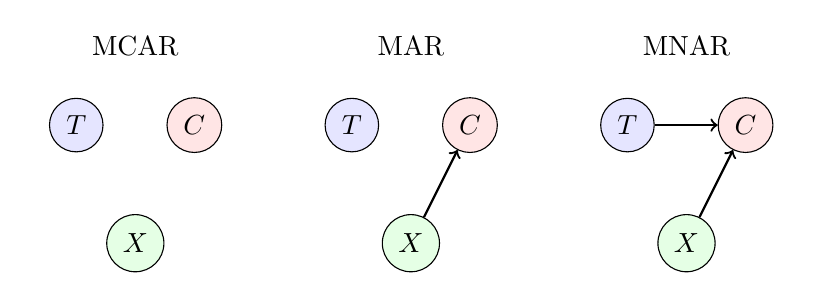
\begin{tikzpicture}
        % MCAR diagram
        \begin{scope}[shift={(-3.5,0)}]
            \node[draw, circle, fill=blue!10] (T1) at (0,0) {$T$};
            \node[draw, circle, fill=red!10] (C1) at (1.5,0) {$C$};
            \node[draw, circle, fill=green!10] (X1) at (0.75,-1.5) {$X$};

            \node[align=center, text width=2.5cm] at (0.75,1) {MCAR};
        \end{scope}

        % MAR diagram
        \begin{scope}[shift={(0,0)}]
            \node[draw, circle, fill=blue!10] (T2) at (0,0) {$T$};
            \node[draw, circle, fill=red!10] (C2) at (1.5,0) {$C$};
            \node[draw, circle, fill=green!10] (X2) at (0.75,-1.5) {$X$};

            \draw[->, thick] (X2) -- (C2);

            \node[align=center, text width=2.5cm] at (0.75,1) {MAR};
        \end{scope}

        % MNAR diagram
        \begin{scope}[shift={(3.5,0)}]
            \node[draw, circle, fill=blue!10] (T3) at (0,0) {$T$};
            \node[draw, circle, fill=red!10] (C3) at (1.5,0) {$C$};
            \node[draw, circle, fill=green!10] (X3) at (0.75,-1.5) {$X$};

            \draw[->, thick] (X3) -- (C3);
            \draw[->, thick] (T3) -- (C3);

            \node[align=center, text width=2.5cm] at (0.75,1) {MNAR};
        \end{scope}
    \end{tikzpicture}
    \caption{Directed acyclic graphs illustrating different censoring mechanisms. Arrows indicate dependencies between variables. Under MCAR, censoring is independent of other variables. Under MAR, censoring depends on observed covariates. Under MNAR, censoring depends on the unobserved event time.}
    \label{fig:censoring-mechanisms}
\end{figure}

\begin{notebox}[title=Non-informative vs. Informative Censoring]
A related distinction is between:
\begin{itemize}
    \item \textbf{Non-informative censoring:} The censoring process provides no information about the event time beyond what is available in the observed covariates (equivalent to MCAR or MAR)
    \item \textbf{Informative censoring:} The censoring process itself provides information about the event time (equivalent to MNAR)
\end{itemize}

Most standard survival methods assume non-informative censoring. When censoring is informative, more complex joint modeling of the censoring and event processes may be required.
\end{notebox}

For survival analysis methods to produce valid results, censoring must typically be:

\begin{itemize}
    \item \textbf{Independent/non-informative:} The censoring mechanism should be unrelated to the event process. If subjects who are more likely to experience the event are also more likely to be censored, we have informative censoring, which can bias results.

    \item \textbf{Random:} The distribution of censoring times should be random and not systematically related to subject characteristics or study conditions.
\end{itemize}

These assumptions should be critically evaluated in any survival analysis. When they're violated, sensitivity analyses or models that account for informative censoring may be needed.

\section{Competing Risks}
\label{sec:competing-risks}

Competing risks occur when subjects can experience multiple types of events, and the occurrence of one event precludes the occurrence of other events or changes their probability. Traditional survival analysis methods that treat competing events as censored can lead to biased estimates.

\begin{figure}[htbp]
    \centering
    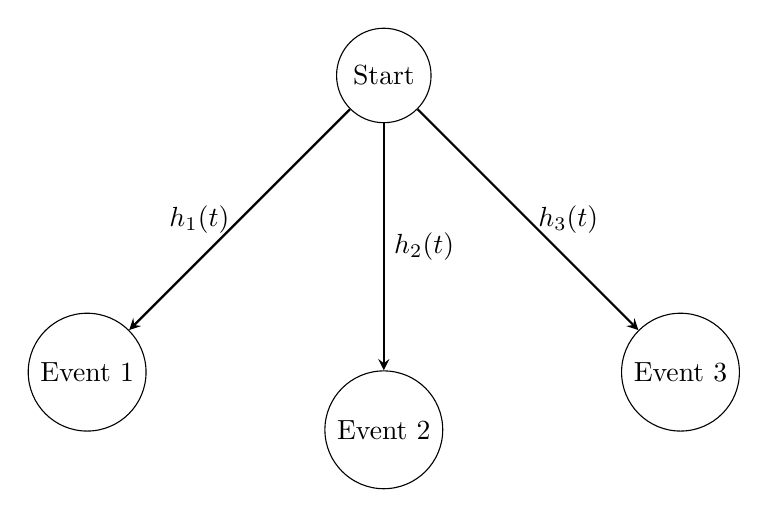
\begin{tikzpicture}[
        node distance=2.5cm,
        state/.style={circle, draw, minimum size=1.2cm},
        arrow/.style={->, >=stealth, thick}
    ]
        % States
        \node[state] (start) at (0,0) {Start};
        \node[state, below left of=start] (event1) at (-2,-2) {Event 1};
        \node[state, below of=start] (event2) at (0,-2) {Event 2};
        \node[state, below right of=start] (event3) at (2,-2) {Event 3};

        % Transitions
        \draw[arrow] (start) -- (event1) node[midway, left] {$h_1(t)$};
        \draw[arrow] (start) -- (event2) node[midway, right] {$h_2(t)$};
        \draw[arrow] (start) -- (event3) node[midway, right] {$h_3(t)$};
    \end{tikzpicture}
    \caption{Competing risks framework. From the initial state, a subject can transition to one of several possible event states, each with its own hazard function. Once one event occurs, the subject is no longer at risk for the other events.}
    \label{fig:competing-risks}
\end{figure}

\subsection{Analyzing Competing Risks}
\label{subsec:analyzing-competing-risks}

When analyzing data with competing risks, we consider:

\begin{itemize}
    \item \textbf{Cause-specific hazards:} The instantaneous rate of occurrence of a specific event type among those still at risk.

    \item \textbf{Cumulative Incidence Function (CIF):} The probability of experiencing a specific event type before time $t$ and before experiencing any competing event.

    \item \textbf{Subdistribution hazard:} The instantaneous rate of occurrence of a specific event type among those who have not experienced that specific event yet (including those who have experienced competing events).
\end{itemize}

Unlike in the standard survival setting where the survival function is directly related to the hazard, in competing risks, the relationship between cause-specific hazards and CIFs is more complex. A reduction in one cause-specific hazard may not necessarily translate to an increase in the corresponding CIF due to the interplay with competing events.

\subsection{Modeling Approaches for Competing Risks}
\label{subsec:modeling-competing-risks}

\begin{itemize}
    \item \textbf{Cause-specific Cox models:} Fit separate Cox models for each cause, treating competing events as censored.

    \item \textbf{Fine and Gray model:} Models the subdistribution hazard directly, allowing for direct assessment of covariate effects on the CIF.

    \item \textbf{Multi-state models:} Consider transitions between different states (e.g., healthy, diseased, dead) and can model complex disease processes.

    \item \textbf{Joint modeling:} Simultaneously model multiple event types, accounting for their dependencies.

    \item \textbf{Neural approaches (e.g., MENSA):} Use neural networks to model complex relationships between covariates and multiple event types.
\end{itemize}

The choice of method depends on the research question—whether the interest is in etiology (cause-specific hazards) or absolute risk prediction (CIFs).

\begin{examplebox}[title=Examples of Competing Risks]
  \begin{itemize}
  \item In medical studies: Death from cancer, heart disease, or other causes
  \item In engineering: Component failure due to wear, corrosion, or manufacturing defect
  \item In business: Customer churn due to price, service quality, or competitor offers
  \item In employment: Job termination due to retirement, new job opportunity, or layoff
  \end{itemize}
\end{examplebox}

\begin{notebox}[title=Important Note on Competing Risks]
A critical point in competing risks analysis is that $1 - S_j(t) \neq F_j(t)$, where $S_j(t)$ is the cause-specific survival function obtained by treating other event types as censored.

The Kaplan-Meier estimator applied to a single event type (treating others as censored) overestimates the probability of that event in the presence of competing risks.
\end{notebox}
